\pstart
Is demum casus resolutus est, quo potentiae\protect\index{Sachverzeichnis}{potentia} ex altera centrorum parte aequidistant a centris ac $C$ restat ut solutio reddatur universalis, exhibere regulam aequilibrii\protect\index{Sachverzeichnis}{aequilibrium} generalem, quae vera sit quocunque potentiarum\protect\index{Sachverzeichnis}{potentia} situ assumto, ibi (inspice figuram \textcjheb{'}) pro  $DE$ et $GH,$ investigandae $de$ et $gh,$ quod ut fiat investigandae \rule[-4mm]{0mm}{10mm}$\displaystyle\frac{DE}{de}$ et $\displaystyle\frac{GH}{gh}$, manifestum est autem esse \rule[-4mm]{0mm}{10mm}$\displaystyle\frac{DR}{dr}=\frac{BD=BC}{BD=BW},$ item esse $\displaystyle\frac{GL}{gl}=\frac{AG=AC}{Ag=AZ}.$ Manifestum est item eodem modo esse item esse \rule[-4mm]{0mm}{10mm}$\displaystyle\frac{ER=CF}{er=\theta\lambda}=\frac{BC=BD}{B\theta=BW}.$  
Item esse \rule[-4mm]{0mm}{10mm}$\displaystyle\frac{H(L)=CF=ER}{hl=\eta\xi}=\frac{AC=AG}{A\eta=Ag=AZ}.$
\pend
\pstart\noindent
\hspace*{0.7cm}Cum ergo sint \rule[-4mm]{0mm}{10mm}$\displaystyle\frac{DR}{dr}=\frac{ER}{er}$\hspace*{0.3cm} erunt et $\displaystyle=\frac{DR-ER=DE}{dr-er=de}=\frac{CF}{\theta\lambda}.$\\
\hspace*{11.5cm}Est autem\\
\hspace*{0.7cm}\edtext{Cum ergo sint}{\lemma{Cum ergo sint [...] erunt et}\Cfootnote{In der Handschrift durch Auslassungsstriche wiedergegeben.}} $\displaystyle\frac{GL}{gl}=\frac{H(L)}{hl}$ erunt et $\displaystyle=\frac{G(L)-H(L)=GH}{gl-hl=gh}=\frac{CF}{\eta\xi}.$
\pend
\vspace*{1mm}
\pstart \noindent
\rule[-4mm]{0mm}{10mm}$\displaystyle\frac{DE}{GH}=\frac{CA^2}{AF\smallfrown AL}=\frac{CF^2+AF^2}{AF\smallfrown AL}.$
Ergo $\displaystyle\frac{DE}{de}\bigtimes\frac{GH}{gh},$ seu $\displaystyle\frac{DEgh}{deGH}$ seu $\displaystyle\frac{DE}{GH}\efrac{\smallfrown}{}\frac{gh}{de}=\frac{CA^2=CF^2+\edtext{\lbrack AF^2\rbrack}{\lemma{}\Bfootnote{$AF$\textit{\ L \"{a}ndert Hrsg.}}}}{AF\smallfrown AL}\efrac{\smallfrown}{}\frac{gh}{de}\overset{\text{est}}=\frac{CF}{\theta\lambda}\bigtimes\frac{CF}{\eta\xi}=\frac{\eta\xi}{\theta\lambda}.$ 
\rule[-4mm]{0mm}{10mm}Ergo $\displaystyle\frac{gh}{de}=\frac{\eta\xi}{\theta\lambda}\efrac{\smallfrown}{}\frac{AF\smallfrown AL}{CA^2}=$\ 
seu ut fiat aequilibrium\protect\index{Sachverzeichnis}{aequilibrium} ratio $B$ ad $A,$ erit composita ex rationibus $\eta\xi$ ad $\theta\lambda$ et (vid. fig. \textcjheb{b}) $AX$ ad $AY.$
Ergo quando ratio $\eta\xi$ ad $\theta\lambda$ est aequalitatis (quod etiam semper fit cum potentiae\protect\index{Sachverzeichnis}{potentia} aequedistant a centris ac centra a vectium\protect\index{Sachverzeichnis}{vectis} contactu,) est \rule[-4mm]{0mm}{10mm}$\displaystyle\frac{B}{A}=\frac{AX}{AY}.$
Et quando $\displaystyle\frac{AF\smallfrown AL}{CA^2}$ est ratio aequalitatis ut fit,
quando $AC$ et $BC$ vectes\protect\index{Sachverzeichnis}{vectis} sibi sunt paralleli et horizontales, (qua tunc $CA=AF=AL$),
tunc \rule[-4mm]{0mm}{10mm}$\displaystyle\frac{B}{A}=\frac{\eta\xi}{\theta\lambda},$ quae ratio ut aestimari possit non cogitandum est $CF$ seu elevationem supra horizontem esse 0, sed = 1, seu infinite parvam.
Ergo erit $\displaystyle\frac{B}{A}=\frac{Ha}{Gf}$\rule[-4mm]{0mm}{10mm}
(insp. fig. \textcjheb{t}) quae $\displaystyle=\frac{Bd}{Bc},$ si $Ba=Bc,$ et $Ef=Ed$ sin inaequalia  ratio $\displaystyle{Ba}{Bc}$ et ratio $\displaystyle\frac{Ef}{Ed}$ compositionem ipsius \rule[-4mm]{0mm}{10mm}$\displaystyle\frac{A}{B}$ impedietur, ut patet.
\pend
\newpage
%\pstart
%\begin{rotate}{90}
%\hspace{-83mm}[\textit{Fig. 5}]
%\end{rotate}
%\pend
%%\vspace{-30mm}
\pstart
\centering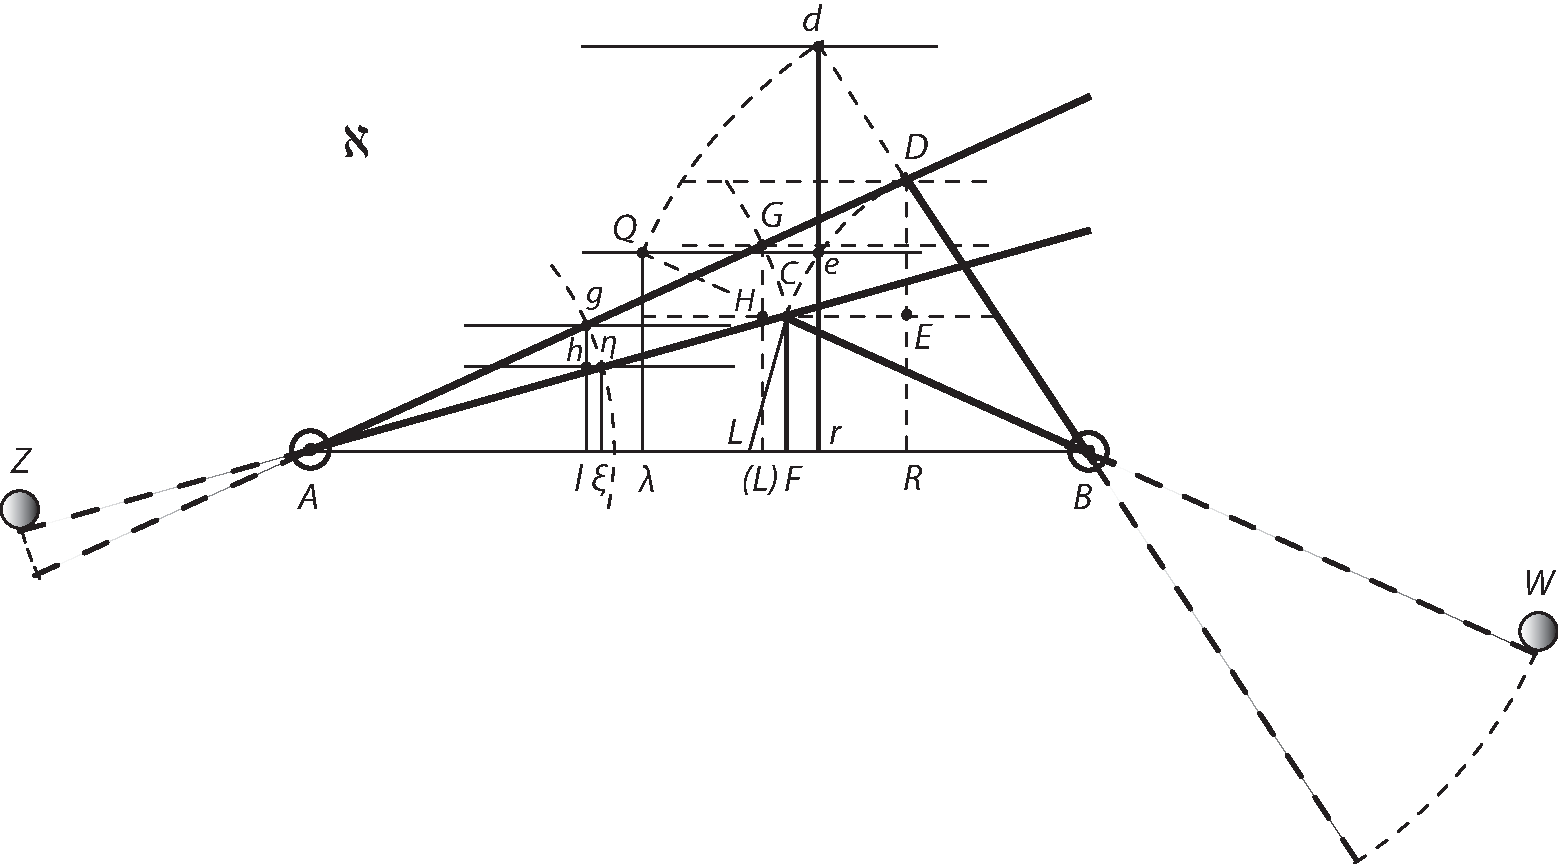
\includegraphics[trim = 0mm 0mm 0mm 0mm, clip,width=1.18\textwidth, angle=90]{images/LH037,03_078r-d1.pdf}
\pend
%\pstart
%\begin{rotate}{90}
%\vspace{70mm}\hspace{80mm}[\textit{Fig. 5}]
%\end{rotate}
%\pend
\vspace{2mm}
\pstart
\centering[\textit{Fig. 5}]
\pend
\count\Afootins=1500
\count\Bfootins=1500
\count\Cfootins=1500
